% In principle, this file can be redistributed and/or modified under
% the terms of the GNU Public License, version 2.


\documentclass{beamer}
\usepackage{adjustbox}
%\usetheme{AnnArbor}
%\usetheme{Antibes}
%\usetheme{Bergen}
%\usetheme{Berkeley}
%\usetheme{Berlin}
%\usetheme{Boadilla}
%\usetheme{boxes}
%\usetheme{CambridgeUS}
%\usetheme{Copenhagen}
%\usetheme{Darmstadt}
%\usetheme{default}
%\usetheme{Frankfurt}
%\usetheme{Goettingen}
%\usetheme{Hannover}
%\usetheme{Ilmenau}
%\usetheme{JuanLesPins}
%\usetheme{Luebeck}
\usetheme{Madrid}
%\usetheme{Malmoe}
%\usetheme{Marburg}
%\usetheme{Montpellier}
%\usetheme{PaloAlto}
%\usetheme{Pittsburgh}
%\usetheme{Rochester}
%\usetheme{Singapore}
%\usetheme{Szeged}
%\usetheme{Warsaw}
\usepackage[utf8]{inputenc}

\title{Prostate Adenocaricome Insights}

\subtitle{Gene Expression approach from TCGA RNA-seq data}

\author{A. Auladell\inst{1}, J. Martí \inst{1} \& D. Mas\inst{1}}

\institute[UPF] 
{
  \inst{1}%
  Department of Experimental \& Health Science\\
  Universitat Pompeu Fabra
}

\date{\today}

\subject{IEO: Information Extraction from Omics technologies}
% This is only inserted into the PDF information catalog. Can be left
% out. 

% If you have a file called "university-logo-filename.xxx", where xxx
% is a graphic format that can be processed by latex or pdflatex,
% resp., then you can add a logo as follows:

\pgfdeclareimage[height=1cm]{upf-logo}{upf.png}
\logo{\pgfuseimage{upf-logo}}

% Delete this, if you do not want the table of contents to pop up at
% the beginning of each subsection:
\AtBeginSection[]
{
  \begin{frame}<beamer>{Outline}
    \tableofcontents[currentsection]
  \end{frame}
}

% Let's get started
\begin{document}

\begin{frame}
  \titlepage
\end{frame}

\begin{frame}{Outline}
  \tableofcontents
  % You might wish to add the option [pausesections]
\end{frame}

% Section and subsections will appear in the presentation overview
% and table of contents.
\section{Introduction}

\subsection{Prostate cancer generalities}
\begin{frame}{Introduction}{Prostate cancer generalities}
  	\begin{block}{Incidence}
		\begin{itemize}
		\item 1 in 7 men will be diagnosed during his lifespan.
		\item 2nd deadliest cancer type in males.
		\item Higher prevalence in African Ancestry.
		\end{itemize}
	\end{block}
	\pause % The slide will pause after showing the first item
	\begin{block}{Previous studies}
		\begin{itemize}
		\item Other RNA-seq studies have been published, most of them at gene level.
		\item The TCGA Consortium gathered a big cohort of patients and have performed several tests and sequencing techniques.
		\end{itemize}
	\end{block}
\end{frame}

\subsection{The Genome Cancer Atlas article}

% You can reveal the parts of a slide one at a time
% with the \pause command:
\begin{frame}{Introduction}{TGCA \cite{Abeshouse2015}}
  \begin{itemize}
  \item<1-> {
    AIM: Create a molecular taxonomy of Prostate Cancer based on 333 tumor samples
    \pause % The slide will pause after showing the first item
  }
  \item<2-> {   
	Data: Whole-exome sequencing (somatic mutations); Array-based methods (somatic copy-number changes); DNA 		methylation and mRNA sequencing (Gene Expression)  
  }
  % You can also specify when the content should appear
  % by using <n->:
  \item<3-> {
    74\% of all tumors were identified in 7 different molecular subtypes: (1) ERG, (2) ETV1, (3) ETV4, or (4) FLI1, (5) SPOP, (6) FOXA1 or (7) IDH1.
  }
  \item<4-> {
  	No relationship between clinical data and molecular cancer subtype (p.e. Gleason score).
  }
  \item<5->{
  	However, subtypes did not share any particular expression pattern. 
  }
  \end{itemize}
\end{frame}

\section{Methods}

\subsection{Data Availability \& Experimental Design}

\begin{frame}{Blocks}
\begin{block}{Block Title}
You can also highlight sections of your presentation in a block, with it's own title
\end{block}
\begin{theorem}
There are separate environments for theorems, examples, definitions and proofs.
\end{theorem}
\begin{example}
Here is an example of an example block.
\end{example}
\end{frame}

\subsection{Processing}


\subsection{Statistical Analysis}



\section{Results}


\subsection{DE genes}

\begin{frame}{Differential Gene Expression}{Volcano Plot}

   \begin{figure}
        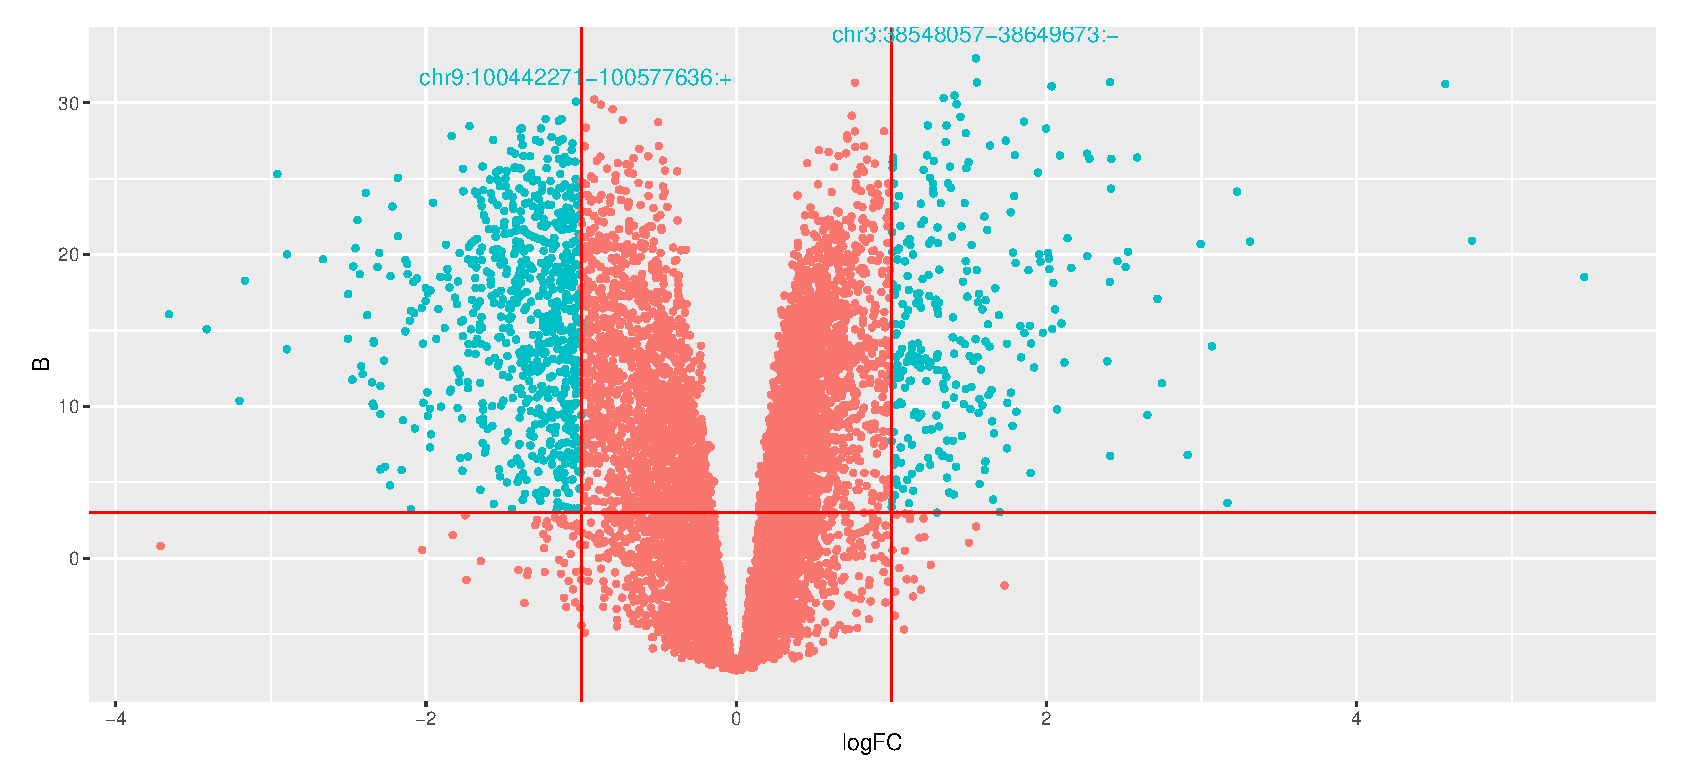
\includegraphics[width=1\textwidth]{Volcano.eps}
    \end{figure}

\end{frame}

\begin{frame}{Differential Gene Expression}{MA plots}

   \begin{figure}
        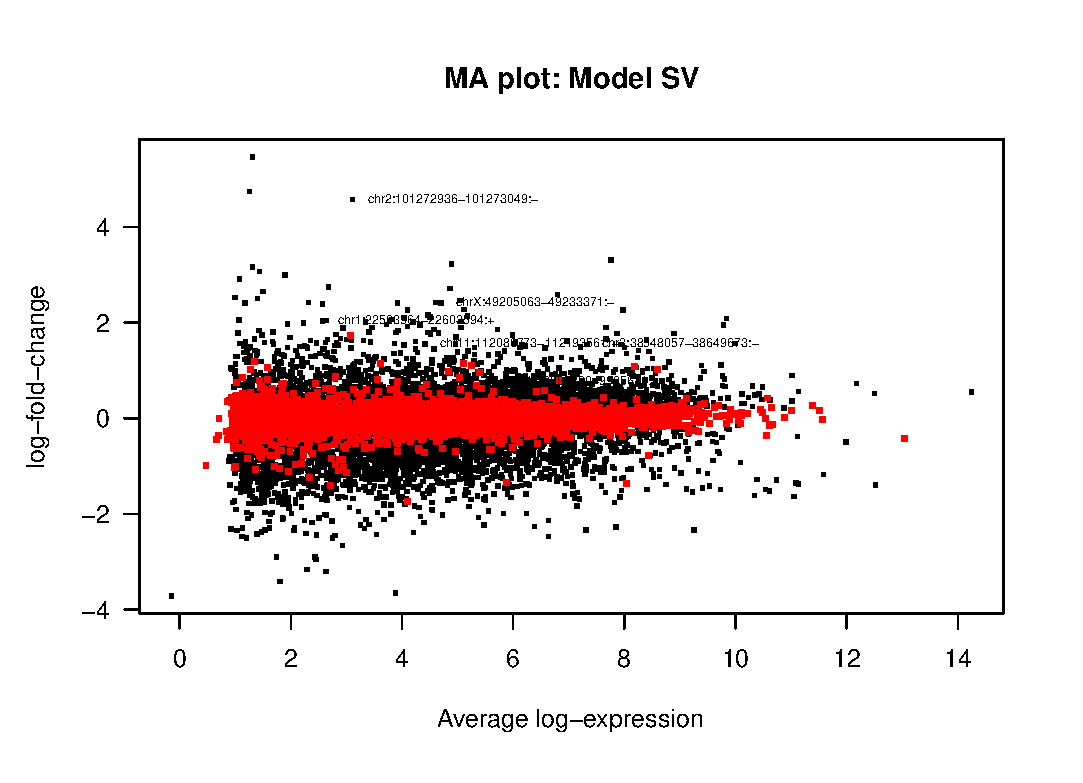
\includegraphics[width=0.8\textwidth,height=0.8\textheight,keepaspectratio]{MAplot.eps}
    \end{figure}

\end{frame}


\begin{frame}{Differential Gene Expression}{Top DE gene}

   \begin{figure}
        \includegraphics[width=0.8\textwidth,height=0.8\textheight,keepaspectratio]{SCN5A}
    \end{figure}

\end{frame}

\begin{frame}{Differential Gene Expression}{Top DE genes}
The Top5 Selected Gene through significance level: \cite{proteinatlas,uhlen2015tissue}
\begin{itemize}
	\item  EPHA8 - ephrin receptor, a neuronal factor.
    \item SNORD89 - small nucleolar RNA.
    \item SCN5A - sodium channel voltage gated V Type.
    \item AP002884.2  - putative gene 
    \item CACNA1F which is a calcium channel voltage dependant L type.
\end{itemize}
\pause
\begin{block}{Neuronal Connection}
Several DE genes present a connection with neuronal processes like EPHA8, SCN5A \& CACNA1F
\end{block}
\pause
\begin{block}{Mapping Error}
The AP002884.2 transcript compromises 2 genes SDHD and BCO2 related with the succinate dehydrogenase with vitamin A biosynthesis.\cite{kent2002human}
\end{block}
\end{frame}

\subsection{Functional Enrichment}
\begin{frame}{Functional Enrichment}{Selected GO terms}
\adjustbox{max width=\textwidth}{

\begin{tabular}{|c|r|r|r|r|r|p{2cm}|p{6cm}|}
 \hline
GOBPID & Pvalue & OddsRatio & ExpCount & Count & Size & Term & Genes \\ 
\hline
GO:0048710 & 0.00 & 11.20 & 7.53 &  13 &  14 & regulation of astrocyte differentiation & DAB1, EPHA4, F2, FGFR3, ATF5, PRPF19, BIN1, HES1, IL1B, NTRK3, SERPINE2, CNTN2, NR2E1 \\ 
GO:0033189 & 0.01 & 9.47 & 6.45 &  11 &  12 & response to vitamin A & DNMT3A, DNMT3B, GATA4, ARG1, LTC4S, RARA, RXRA, TSHB, TYMS, CAT, ALDH1A2 \\ 
 GO:0032309 & 0.01 & 6.03 & 8.60 &  14 &  16 & icosanoid secretion & ABCC4, ACE, DRD3, AGTR2, ACSL4, ANXA1, IL1B, NTSR1, OXT, P2RX7, BDKRB2, SYK, CYP4F2, TNFSF11 \\ 
GO:1901571 & 0.01 & 4.31 & 9.68 &  15 &  18 & fatty acid derivative transport & ABCC4, ACE, DRD3, AGTR2, ACSL4, ANXA1, IL1B, NTSR1, OXT, P2RX7, BDKRB2, SLCO2A1, SYK, CYP4F2, TNFSF11 \\ 
GO:0043966 & 0.01 & 3.45 & 13.45 &  20 &  25 & histone H3 acetylation & TRIM16, TAF6L, WDR5, CHEK1, KAT7, SGF29, DR1, BRD4, KAT6B, WBP2, SIN3A, BRPF3, PER1, PIH1D1, CSRP2BP, BRCA2, TAF10, BRPF1, KAT2B, SUPT7L \\ 
   \hline
\end{tabular}

}
\end{frame}

\subsection{Gene Set Expression Analysis}


\begin{frame}{Gene Set Expression Analysis}{ Enrichment approach (GSEA)}
\adjustbox{max width=\textwidth}{
\begin{tabular}{|l|c|c|p{6.3cm}|}
 \hline
Gene Set & Relative tumor expression &  Z-value & Genes \\
  \hline
REACTOME DEADENYLATION OF MRNA & Over-Expressed  & 19.19 & EIF4A1, EIF4A2, EIF4B, EIF4E, EIF4G1, CNOT2, CNOT4, RQCD1, CNOT8, PAN2, CNOT1, CNOT10, PABPC1, CNOT7, CNOT6, TNKS1BP1, CNOT6L, PAN3 \\
REACTOME SMOOTH MUSCLE CONTRACTION & Under-Expressed & 18.70 & ACTA2, ACTG2, CALM1, CALM3, ITGA1, ITGB5, PXN, TPM2, VCL, SORBS1 \\
REACTOME BOTULINUM NEUROTOXICITY & Over-Expressed &  17.62 & SNAP25, SYT1, STX16, STX11, STX10, STX6, STX12, STX1B \\
REACTOME ENDOGENOUS STEROLS & Under-Expressed & 17.54 & CYP8B1, CYP11B1, CYP51A1, CYP46A1, CYP39A1 \\
\hline
\end{tabular}
}
\end{frame}

\begin{frame}{Gene Set Expression Analysis}{ Enrichment approach (GSEA)}
\centering 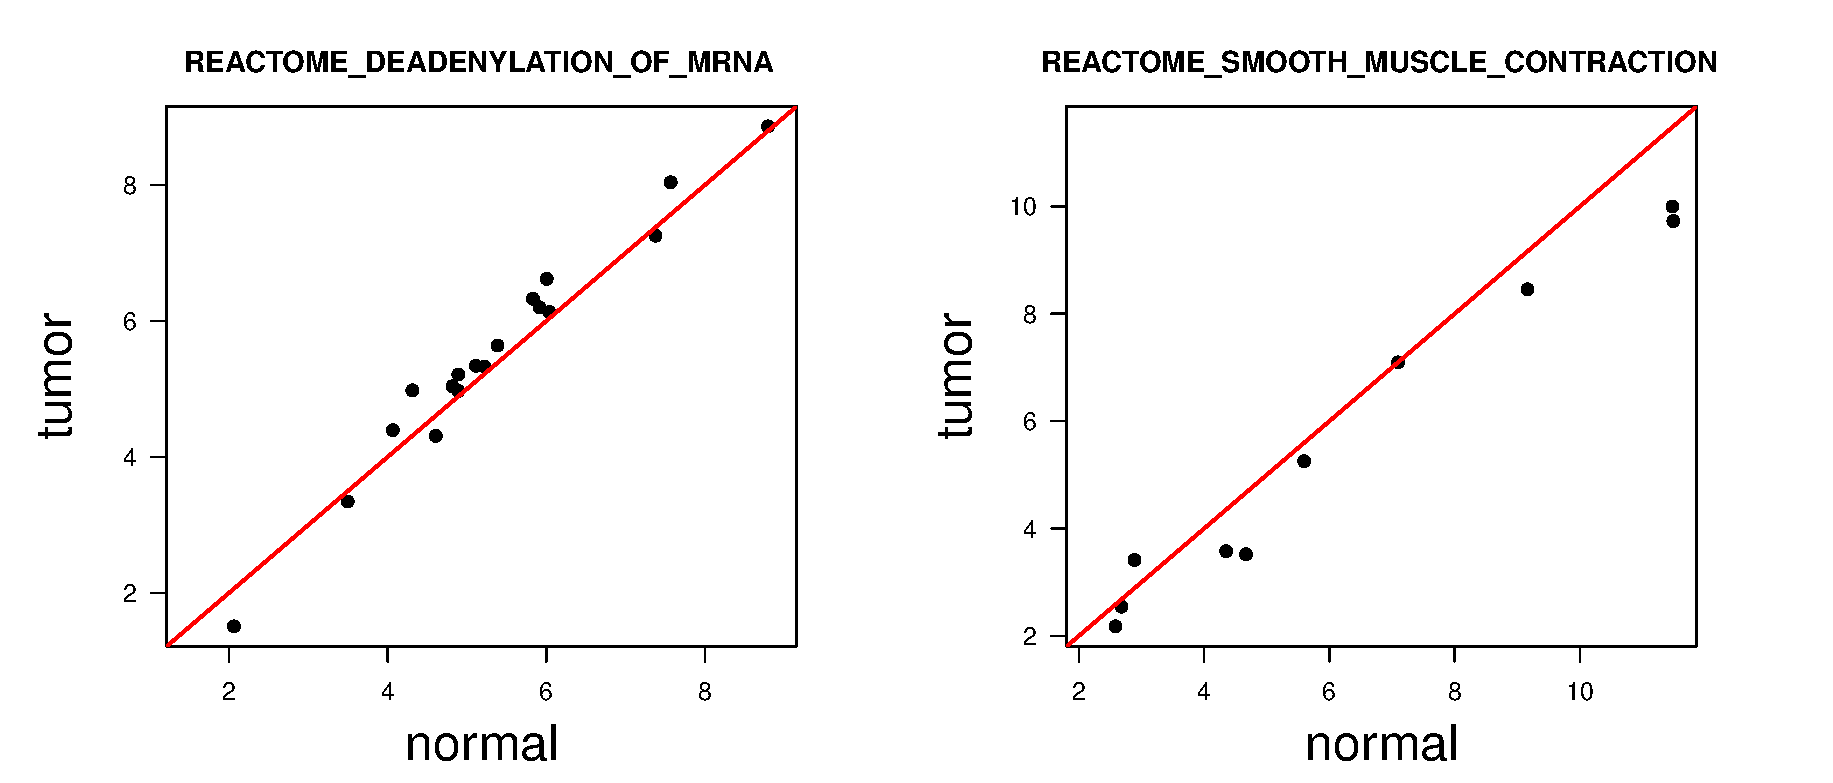
\includegraphics[width=0.8\textwidth,height=0.4\textheight,keepaspectratio]{genesets1.eps} \\
        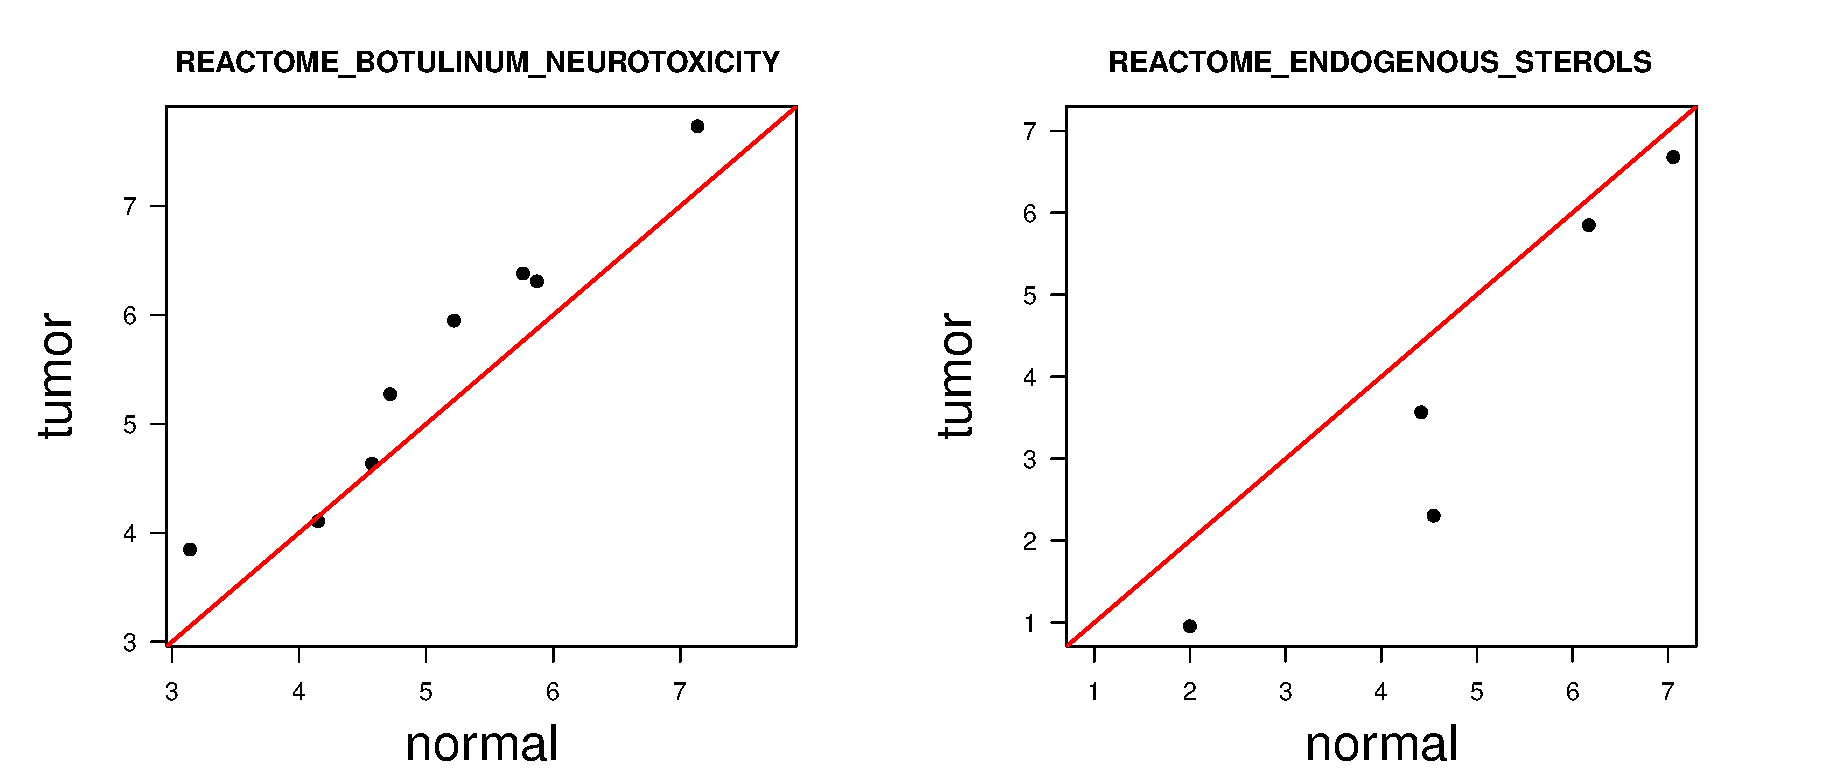
\includegraphics[width=0.8\textwidth,height=0.4\textheight,keepaspectratio]{genesets2.eps}
\end{frame}

\begin{frame}{Gene Set Expression Analysis}{ Variation  approach (GSVA)}
   \centering
        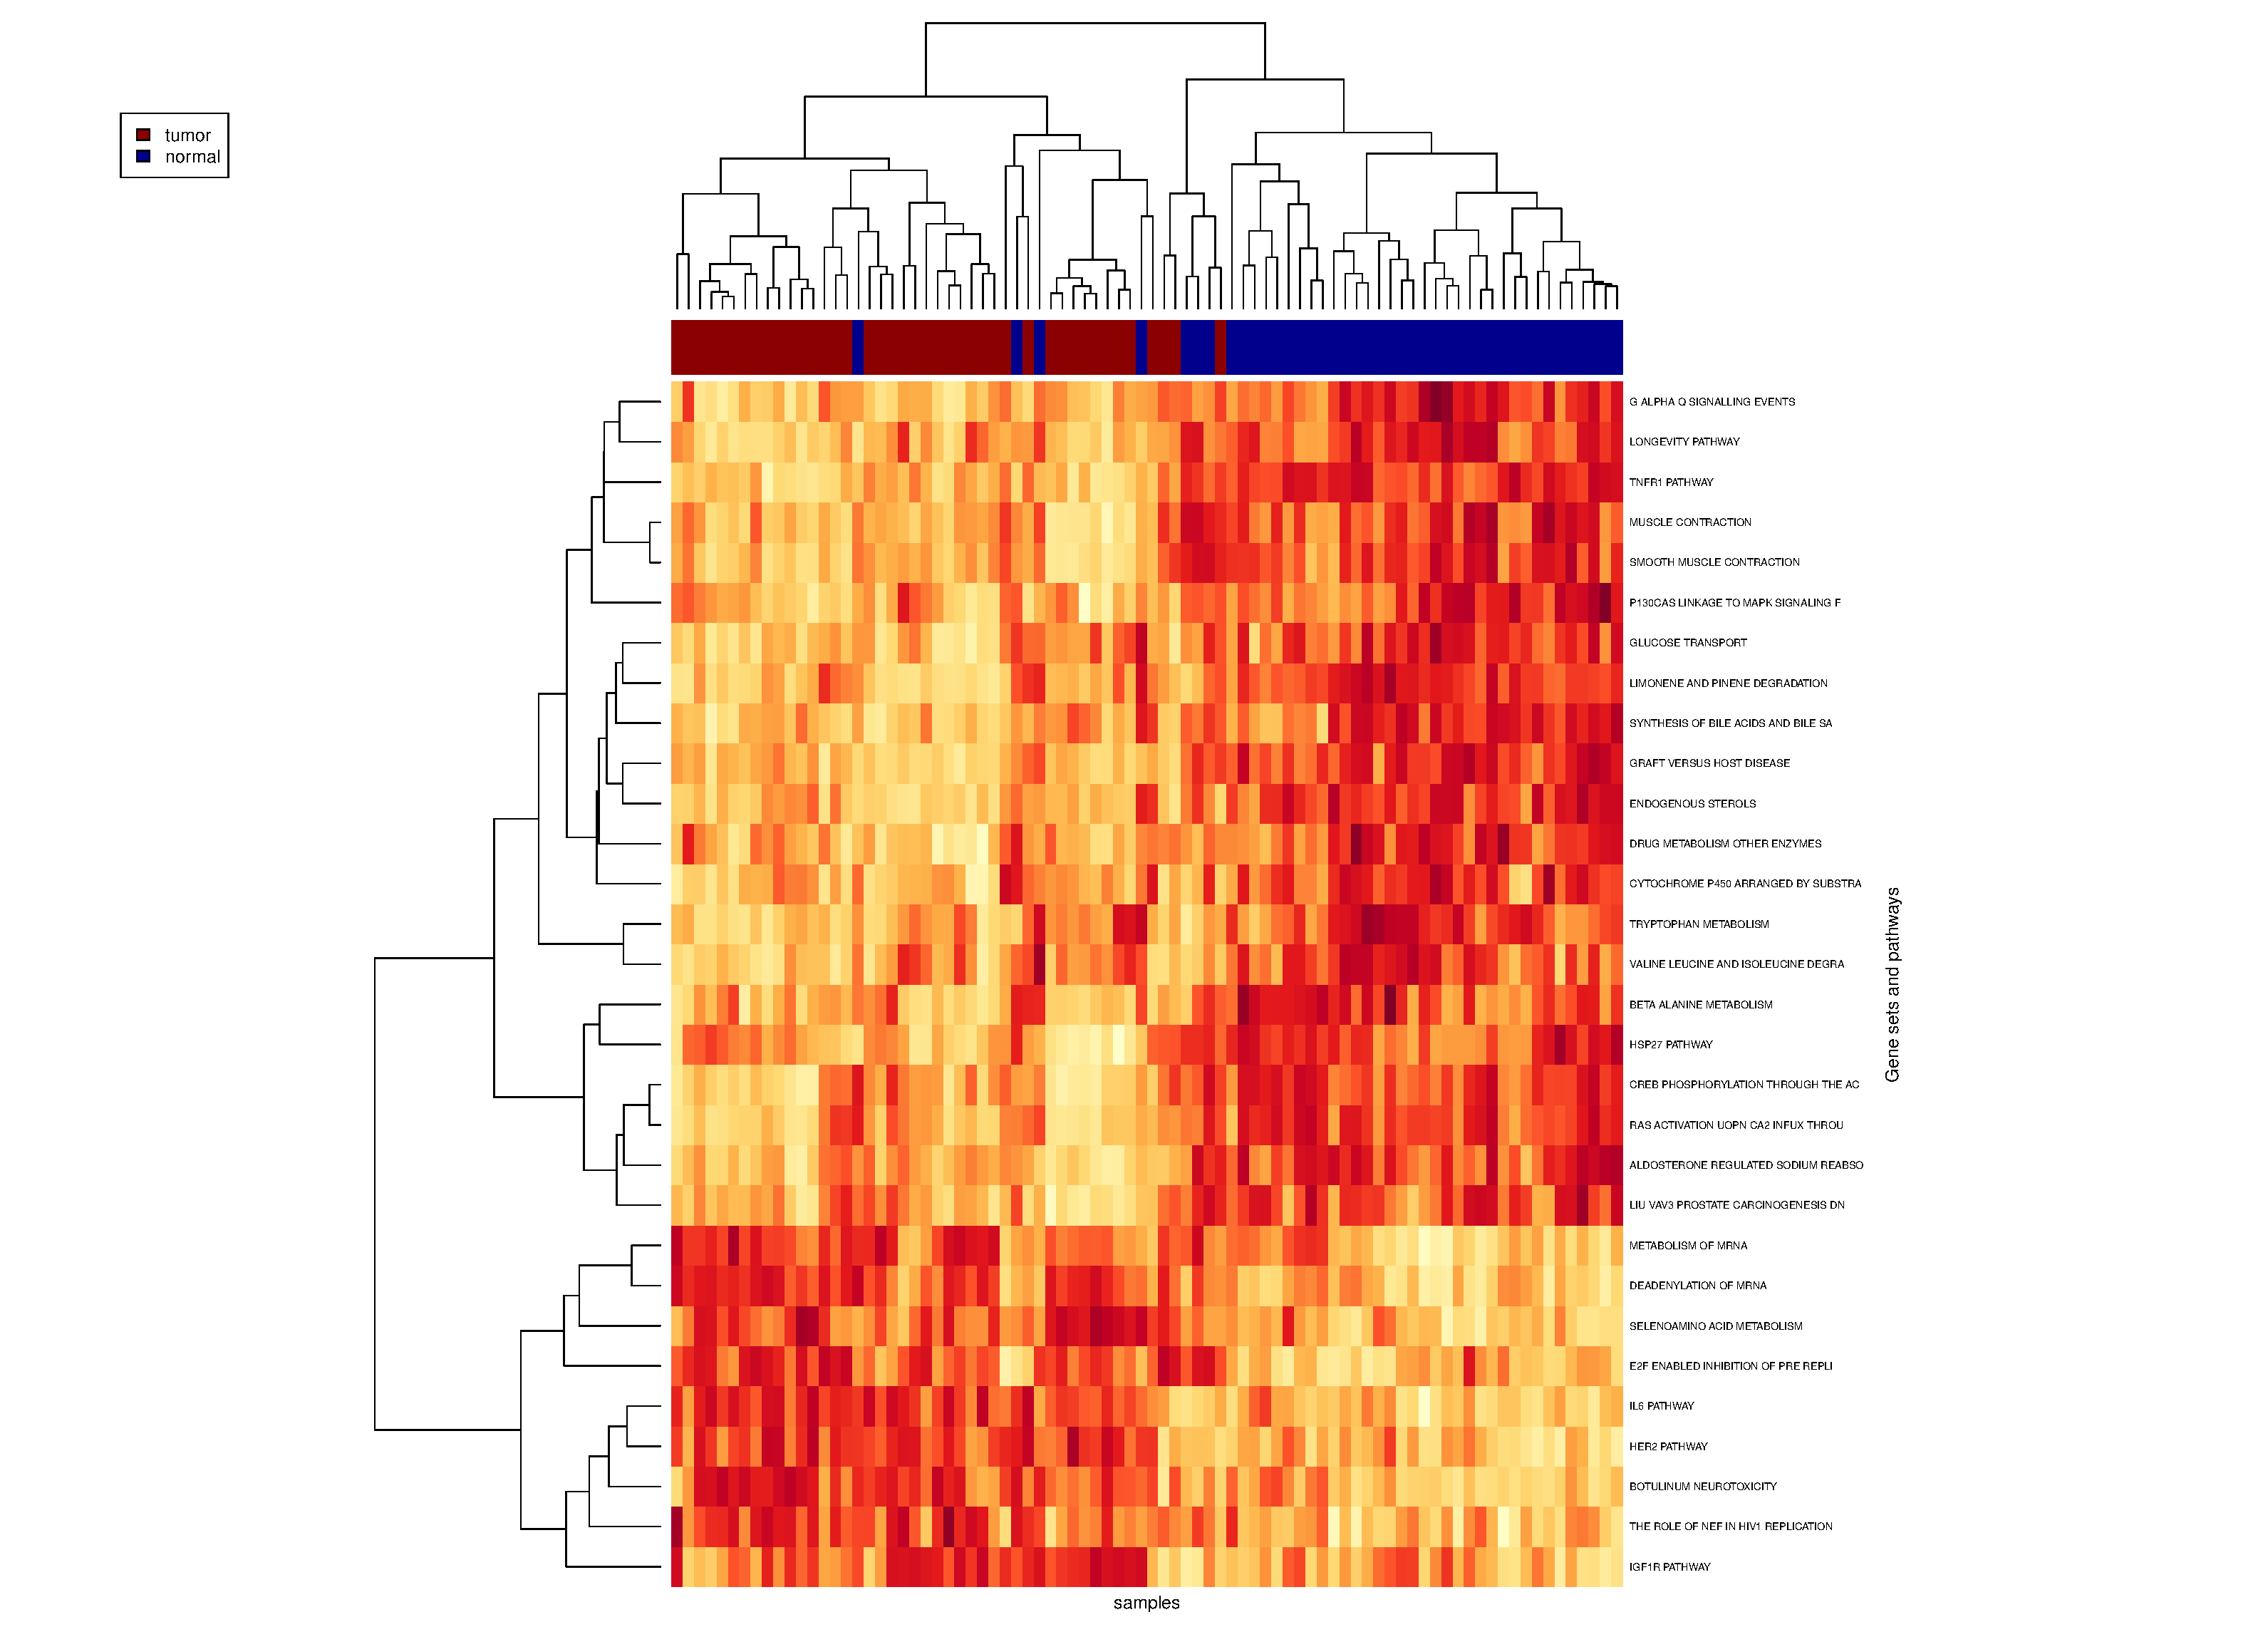
\includegraphics[width=1\textwidth,height=0.8\textheight,keepaspectratio]{ClusteringGSVA.eps}

\end{frame}


\begin{frame}{Gene Set Expression Analysis}{ Comparison}
\centering
        \includegraphics[width=.7\textwidth,height=0.8\textheight,keepaspectratio]{venn}
\end{frame}




\section{Conclusions}

\begin{frame}{Summary}
  \begin{itemize}
  \item
    The \alert{first main message} of your talk in one or two lines.
  \item
    The \alert{second main message} of your talk in one or two lines.
  \item
    Perhaps a \alert{third message}, but not more than that.
  \end{itemize}
  
  \begin{itemize}
  \item
    Outlook
    \begin{itemize}
    \item
      Something you haven't solved. 
    \item
      Something else you haven't solved.
    \end{itemize}
  \end{itemize}
\end{frame}



% All of the following is optional and typically not needed. 
\appendix
\section<presentation>*{\appendixname}
\subsection<presentation>*{For Further Reading}


\begin{frame}[allowframebreaks]%in case more than 1 slide needed
\frametitle<presentation>{References}
    {\footnotesize
    \bibliographystyle{unsrt}
    \bibliography{prac-bibliography}
    }
\end{frame}


\end{document}


